\UseRawInputEncoding
\chapter{Metodología}
En este capítulo se describirá la forma en la que se ha trabajado durante el desarrollo del proyecto.
El marco del desarrollo será el {\href{https://www.redhat.com/es/topics/devops/what-is-agile-methodology}{desarrollo ágil}}; que se centra en el usuario, por lo que se utilizará una planificación ágil, con el objetivo
de conseguir un software de calidad y flexible. Esto debe estar presente constantemente en el desarrollo del proyecto.

\section{Planificación}
La planificación que se va a emplear está basada en los {\href{https://agilemanifesto.org/iso/es/principles.html}{principios del manifiesto ágil}}
Buscamos un tipo de planificación que se centre en el usuario, para que el propio usuario nos aporte retroalimentación, aunque para este caso no sea posible por la
ausencia de un cliente real, por lo que debemos de escoger una planificación específica. En mi caso he usado Kanban con la ayuda del tablero de GitHub.

\begin{figure}[h]
    \centering
    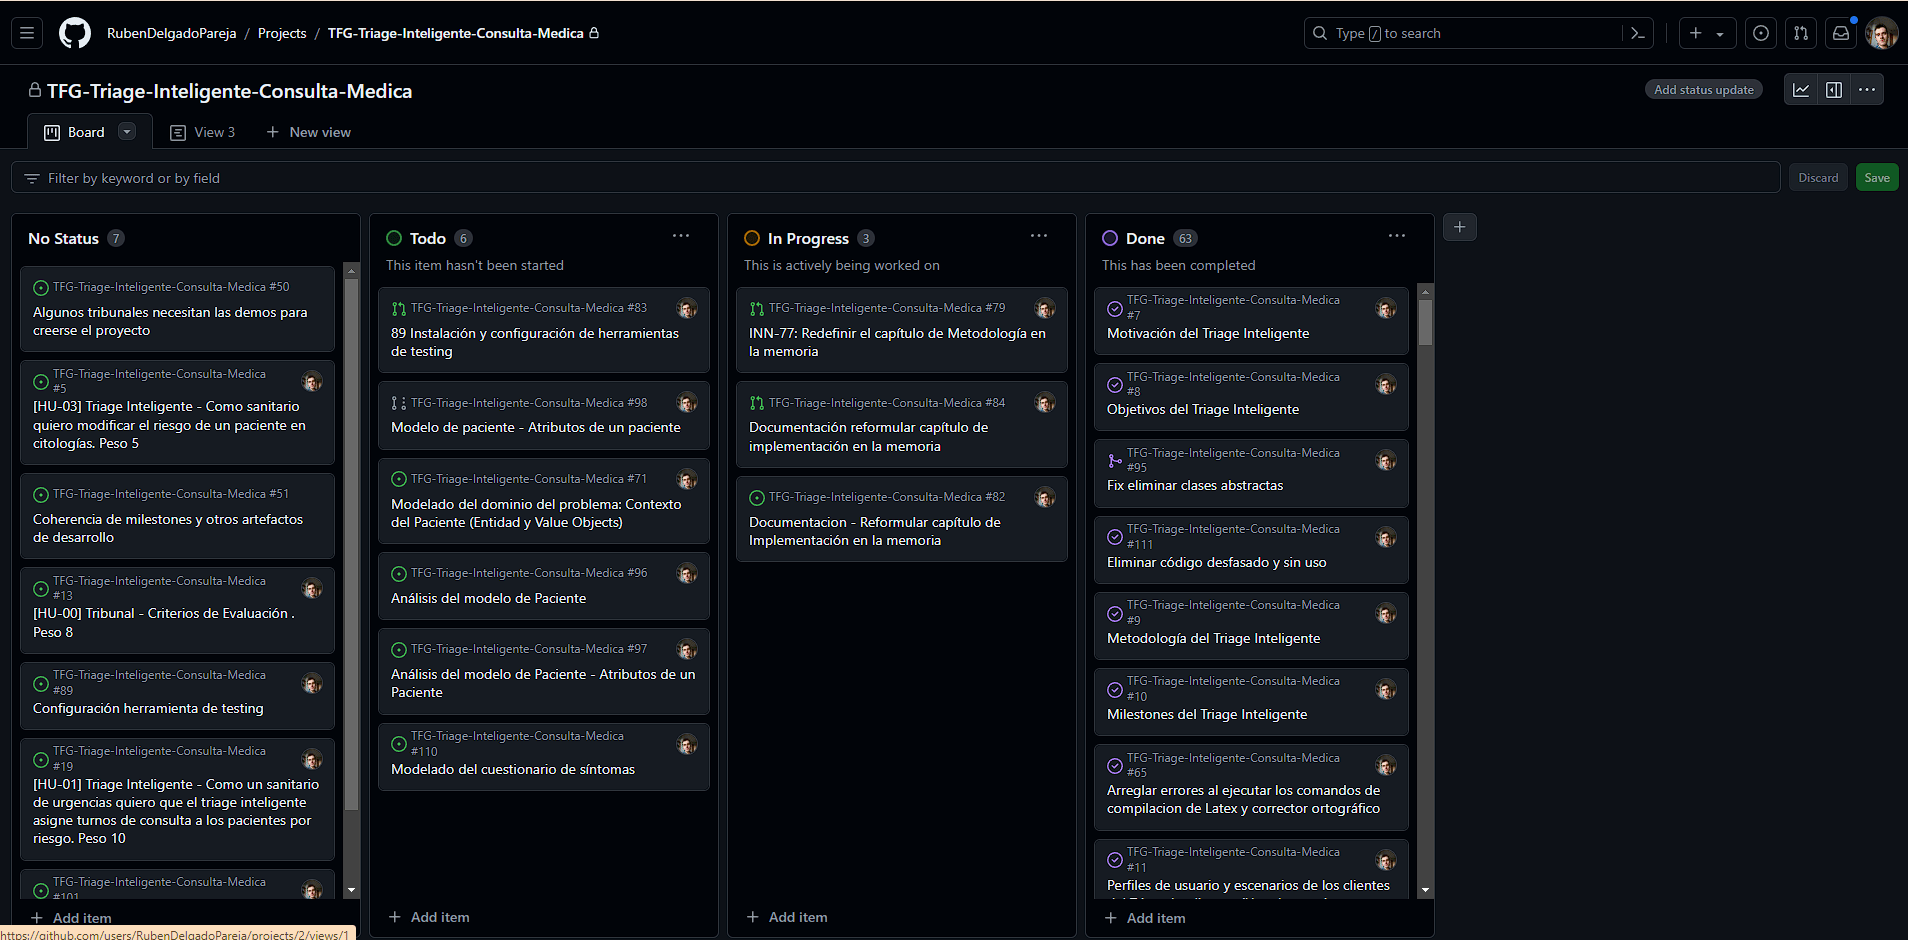
\includegraphics[width=0.9\linewidth]{logos/kanban.png}
    \caption{Tablero Kanban.}
    \label{fig:layout1}
\end{figure}

Una planificación ágil nos permite adaptarnos al cambio de requisitos haciendo uso de las iteraciones y aprovechar las nuevas oportunidades que aparezcan.
El desarrollo ágil construye el sistema por medio de aportaciones frecuentes de código que aportan valor
al usuario, es necesario organizar las funcionalidades en bloques y que los cambios siempre surgen de una necesidad del usuario.

\section{Análisis de usuarios}
Dentro del marco de desarrollo ágil, comprender las necesidades y experiencias de los usuarios es fundamental para el éxito del proyecto.
En esta sección, nos adentramos en el concepto de User Journeys, una herramienta para entender cómo interactúan los usuarios con nuestro producto o servicio a lo largo de su ciclo de vida.

\UseRawInputEncoding
\section{\textit{User Journeys}}\label{anexo}

\subsection{Rafael González Pérez}
\begin{itemize}
    \item \textbf{Contexto de uso: }
    \begin{itemize}
        \item \textbf{¿Cuándo utiliza el ordenador?: }  Utiliza el ordenador con frecuencia
        \item \textbf{¿Dónde utiliza el ordenador?: } En el trabajo y en casa
        \item \textbf{¿Qué tipo de ordenador utiliza?: } El ordenador de la consulta de urgencias
    \end{itemize}
    \item \textbf{Misión: }
    \begin{itemize}
        \item \textbf{¿Para qué quiere utilizar nuestra aplicación?: } Como sanitario de urgencia quiero priorizar los pacientes con mayor riesgo
        \item \textbf{¿Qué espera encontrar en ella?: } Una aplicación web con el triage de urgencias que organice los turnos de los pacientes
    \end{itemize}
    \item \textbf{Motivación: }
    \begin{itemize}
        \item \textbf{¿Para cuándo quiere utilizarla?: } Cuando comience su jornada laboral en el hospital
        \item \textbf{¿Por qué quiere alcanzar ese objetivo?: } Para automatizar el proceso del triage
    \end{itemize}
    \item \textbf{Actitud hacia la tecnología: } Se siente cómodo navegando por Internet y usando las nuevas tecnologías. No le es ningún impedimento
\end{itemize}

\subsection{Escenario 1 de Rafael González Pérez}
    Rafael es un sanitario que trabaja de guardias en un hospital de urgencias. Rafael se encarga
    de gestionar los pacientes que llegan a urgencias y a través de una pequeña entrevista con el paciente asignarle
    una prioridad u orden de consulta. Rafael descubre que en otros hospitales utilizan un sistema de triage inteligente
    que les ayuda a priorizar a los pacientes y a organizar los turnos de los pacientes. Rafael propone implantarlo en su hospital.
    Rafa consigue implantar el nuevo triage inteligente y lo pone en práctica en su jornada laboral. Los pacientes que van llegando
    a urgencias realizan el cuestionario del triage y automáticamente se les asigna un nivel de prioridad y un tiempo de demora estimado.
    Él puede ver en su pantalla los pacientes que están en espera y el tiempo estimado que les queda para ser atendidos. En caso
    de que sea necesario, Rafa puede asignar manualmente un nivel de prioridad a un paciente en concreto bajo su propio criterio.
    Gracias al triage inteligente, puede organizar los turnos de los pacientes de forma eficiente y rápida.


\subsection{Azucena Rodríguez Peralta}
\begin{itemize}
    \item \textbf{Contexto de uso: }
    \begin{itemize}
        \item \textbf{¿Cuándo utiliza el ordenador?: }  Usa el ordenador a diario
        \item \textbf{¿Dónde utiliza el ordenador?: } En casa y en el trabajo
        \item \textbf{¿Qué tipo de ordenador utiliza?: } El ordenador que le ofrecen en la consulta
    \end{itemize}
    \item \textbf{Misión: }
    \begin{itemize}
        \item \textbf{¿Para qué quiere utilizar nuestra aplicación?: } Para citar con antelación a los pacientes con mayor posibilidad de diagnóstico.
        \item \textbf{¿Qué espera encontrar en ella?: } Una web sencilla para saber cuando tiene cita con sus pacientes y los riesgos / síntomas que presentan.
    \end{itemize}
    \item \textbf{Motivación: }
    \begin{itemize}
        \item \textbf{¿Para cuándo quiere utilizarla?: } Para el trabajo
        \item \textbf{¿Por qué quiere alcanzar ese objetivo?: } Porque quiere diagnosticar posibles enfermedades lo antes posible
    \end{itemize}
    \item \textbf{Actitud hacia la tecnología: } Está muy acostumbrada a usar un ordenador
\end{itemize}

\subsection{Escenario Azucena Rodríguez Peralta}
    Azucena es una mujer que ha estudiado la carrera de Enfermería y está especializada en matrona.
    Acaba de mudarse a una nueva ciudad, donde comenzará a trabajar como matrona de consulta. Azucena se encarga
    de las consultas a cerca del cáncer de cuello de útero donde se presupone un paciente sano, por lo que cita
    a sus pacientes con bastante demora. Con frecuencia, Azucena tiene que atender a pacientes que muestran sintomas
    alarmantes que dan indicios al diagnóstico del cáncer, por lo que propone usar un nuevo sistema de triage inteligente.
    La web le permite a Azucena organizar las citas de sus pacientes y priorizar a los pacientes con mayor riesgo.
    Cuando un paciente recibe una cita con Azucena, este tiene que rellenar un cuestionario con sus síntomas alarmantes.
    Los pacientes con síntomas preocupantes son priorizados y citados con antelación. En caso de un diagnóstico precoz,
    Azucena podrá manualmente cambiar el riesgo del paciente para no tenga tanta demora como los pacientes sanos.
    Gracias al triage inteligente, Azucena puede llegar a diagnosticar enfermedades de forma precoz y rápida.


\section{Control de versiones}
Una herramienta de control de versiones ayuda a un desarrollo iterativo, en el que se compruebe el trabajo constantemente indispensable para el desarrollo ágil.
La herramienta que yo he escogido es git y GitHub por su facilidad de uso y por su integración con otras herramientas.
Soy consciente de que existen otras herramientas como GitLab o Bitbucket, pero GitHub es muy buena opción, ya que, es gratuita, la más utilizada y tiene una gran comunidad.

\section{Hitos}
El desarrollo ágil debe ser incremental y para ello se debe dividir la carga de trabajo de diferentes hitos.
Los hitos pueden definirse como metas a las que debemos de llegar durante el desarrollo del proyecto.
Los hitos son una buena forma de limitar los bloques de trabajo del desarrollo y su principal intención es que
al final de cada hito consigamos un producto mínimamente viable (\textit{PMV}) para que sea independiente e iterativo.
Durante el desarrollo de un hito surgen las \textit{issues}.

\subsection{Issues}
Las issues son problemas que van surgiendo durante el desarrollo del hito y
el conjunto de las soluciones de las issues de un hito deben conformar el PMV que satisfaga la necesidad del usuario.
Las issues deben hacer referencia a una historia de usuario, ya sea para solucionar un problema de la propia historia o para añadir una funcionalidad.
Todas las Issues que solucionaré durante el desarrollo para construir el sistema están descritas en GitHub. Cada issue debe tener mínimo un commit asociado a su
etiqueta y debe tener una pull request asociada para poder revisar el código.

\begin{figure}[!tb]
    \begin{center}
        \subfigure[Listado de issues.]{
            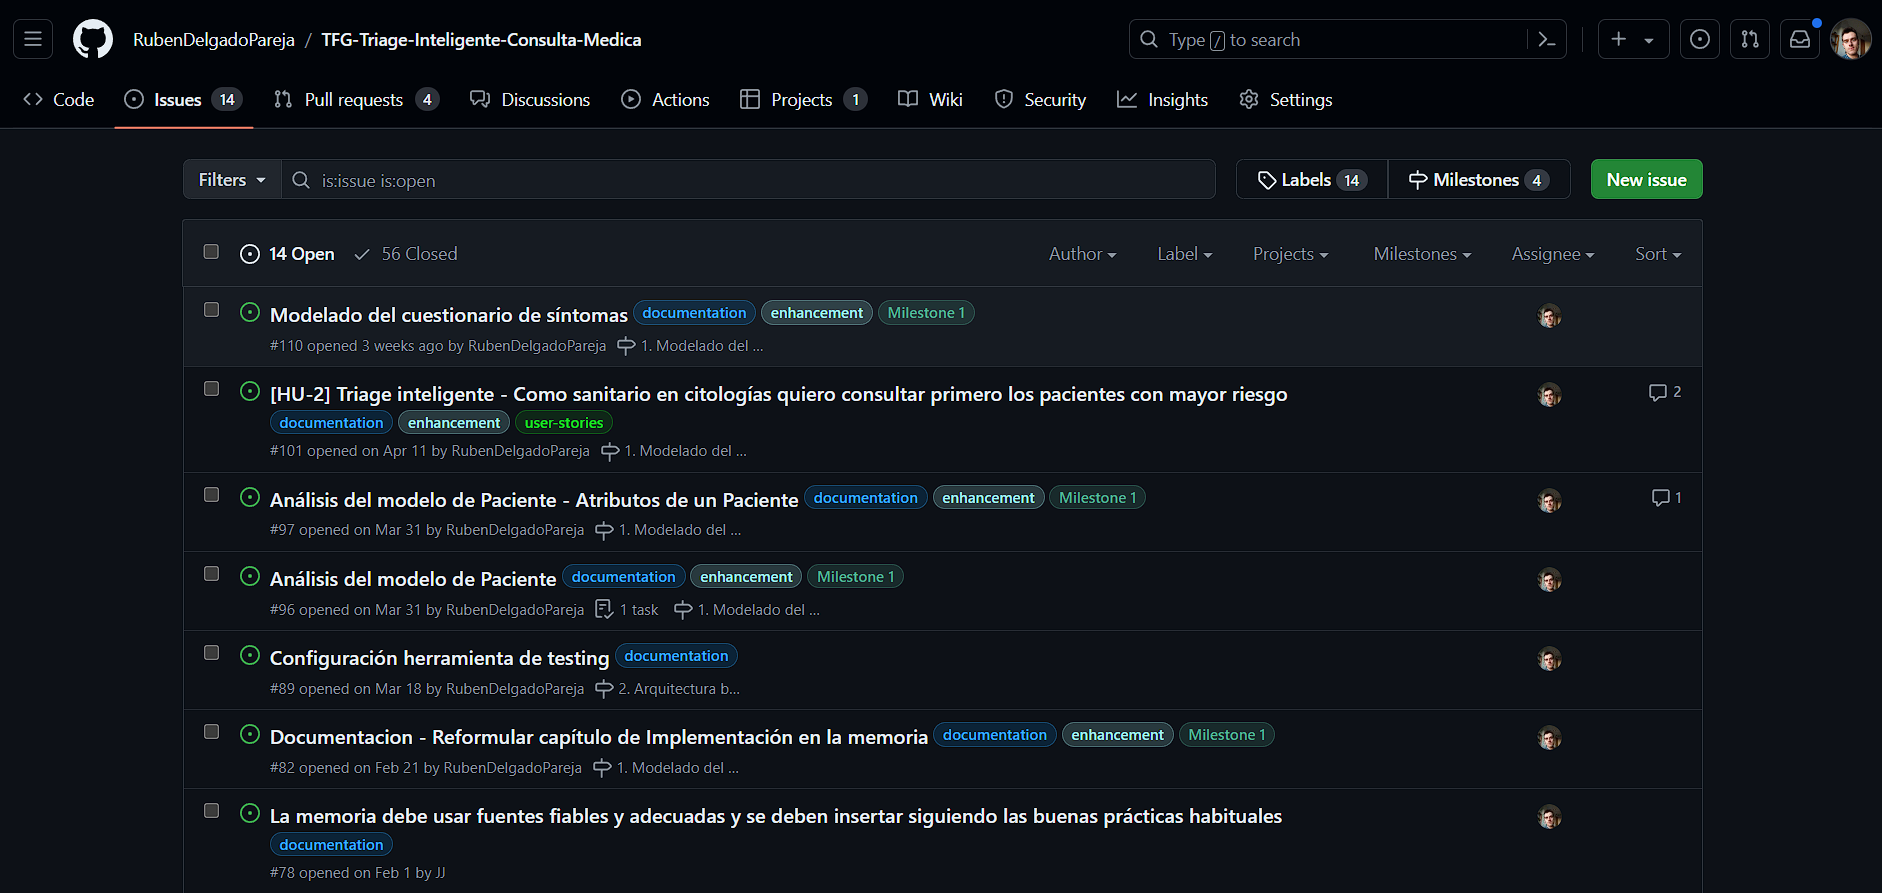
\includegraphics[width=0.9\linewidth]{logos/issues.png}
            \label{Imagen-Issues}}
        \subfigure[Listado de Pull Requests.]{
            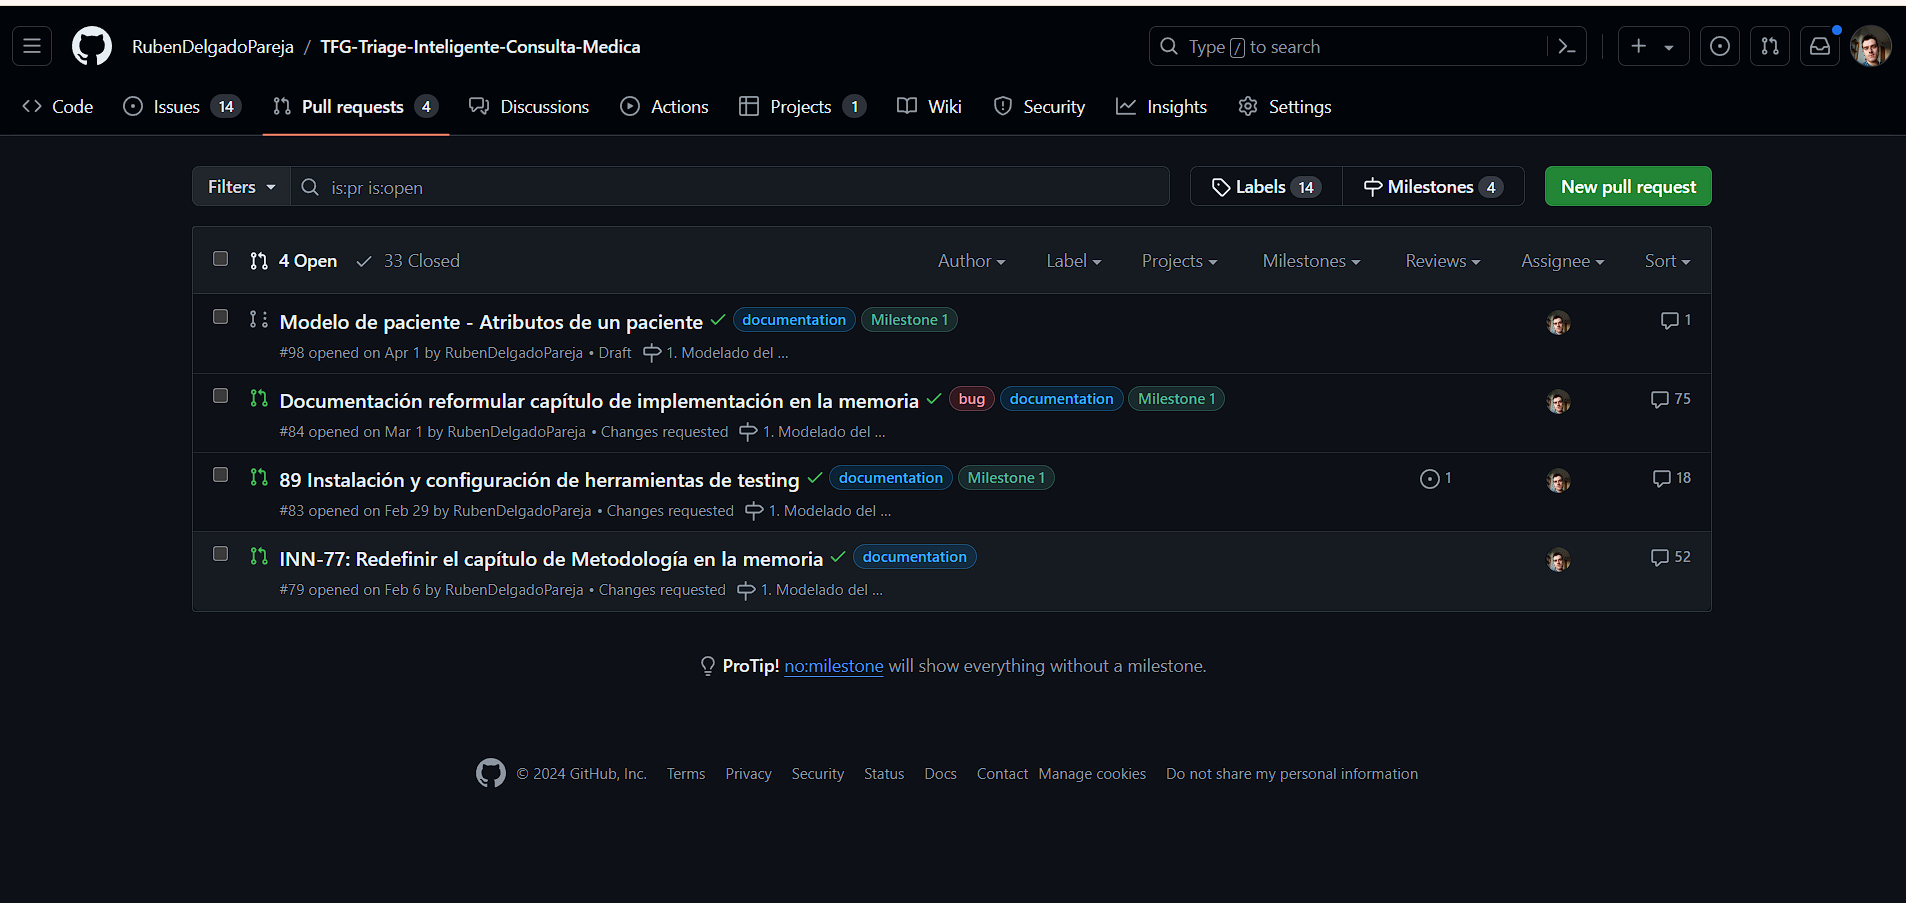
\includegraphics[width=0.9\linewidth]{logos/pullrequest.png}
            \label{Imagen-PullRequests}}
        \label{Figura-Ciudades}
    \end{center}
\end{figure}


Los hitos que se deben de cumplir están reflejados en el GitHub y son los siguientes:

\subsection*{\href{https://github.com/RubenDelgadoPareja/TFG-Triage-Inteligente-Consulta-Medica/milestone/1}{Hito 0: Infraestructura inicial y documentación}}

El primer PMV consiste en alcanzar un repositorio inicial donde comenzar a forjar toda la arquitectura del proyecto con una planificación inicial.
Para aceptar el PMV, el repositorio debe de contener:

\begin{itemize}
    \item{User Journeys.}
    \item{Hitos.}
    \item{Historias de Usuario.}
    \item{Comprobadores de gramática y ortografía.}
    \item{Comprobadores de compilación de LaTeX para la documentación.}
    \item{Documentar las secciones de Motivación, Objetivos y Planificación}
\end{itemize}

\subsection*{\href{https://github.com/RubenDelgadoPareja/TFG-Triage-Inteligente-Consulta-Medica/milestone/7}{Hito 1: Modelado del Problema con DDD}}

Este PMV consiste en modular el dominio del problema para facilitar el diseño e implementación.
Para aceptar el PMV la memoria debe de recoger una sección específica sobre cómo se aplicará el DDD la cual incluya:

\begin{itemize}
    \item {Definición del dominio}
    \item {Definir el lenguaje ubicuo}
    \item {Identificar Entities, Value Objects, Aggregates}
    \item {Definir los Repositories y Services necesarios}
\end{itemize}


\subsection*{\href{https://github.com/RubenDelgadoPareja/TFG-Triage-Inteligente-Consulta-Medica/milestone/2}{Hito 2: Arquitectura básica del sistema de colas de citas}}

Este PMV consiste en diseñar las clases y funciones necesarias para crear citas, almacenarlas en colas y priorizarlas mediante una heurística.

Los criterios de aceptación de este PMV son los tests de cada clase y sus funciones, además de reflejar en la memoria las decisiones tomadas

\section{Historias de Usuarios}
Este concepto es fundamental en el desarrollo ágil, ya que, resume las necesidades del usuario.
Las historias de usuario son la unidad mínima de funcionalidad que el usuario necesita del sistema, es decir,
expresa lo que quiere el usuario del sistema por esto lo hace tan importante, se centra completamente en el
usuario. Encontraremos las Historias de Usuario repartidas por los Hitos del desarrollo del software.

\noindent{Se han definido las siguientes historias de usuario:}

\subsection*{\href{https://github.com/RubenDelgadoPareja/TFG-Triage-Inteligente-Consulta-Medica/issues/19}{[HU-01] Triage Inteligente - Como sanitario de urgencias quiero que el triage inteligente asigne turnos de consulta automáticamente por riesgo.}}
Como sanitario de urgencias quiero un sistema de triage inteligente que se encargue de aplicar un cribado de riesgos a los pacientes.
El triage se encarga de evaluar el estado de salud del paciente a través de un formulario dónde se le pregunta al paciente el motivo de la consulta y
síntomas que padece, con esta información el sistema le asignará un riesgo de los cinco niveles establecidos, dependiendo del riesgo el paciente tendrá una demora
específica de tiempo para ser atendido. En caso de que supere el tiempo de demora y no sea atendido se podrá reevaluar el riesgo del paciente.
El triage funcionará todo el día y puede tener supervisión de un sanitario en todo momento, este sanitario podría, según su criterio cambiar el riesgo del paciente.

\subsection*{\href{https://github.com/RubenDelgadoPareja/TFG-Triage-Inteligente-Consulta-Medica/issues/101}{[HU-02] Triage Inteligente - Como sanitario de citología quiero consultar los pacientes con mayores riesgos.}}
Como sanitario de citologías quiero un sistema de triage inteligente que se encargue de aplicar un cribado de riesgos a los pacientes con mayor riesgo.
El triage inteligente en citología estará enfocado a la propia citología, por lo que se tratará de un cuestionario acerca de posibles síntomas alarmantes
que den indicios de la enfermedad. En citología, la demora de consulta es muy alta, por lo que la diagnosis precoz es fundamental para el paciente.

\subsection*{\href{https://github.com/RubenDelgadoPareja/TFG-Triage-Inteligente-Consulta-Medica/issues/5}{[HU-03] Triage Inteligente - Como sanitario de citología quiero modificar el riesgo de un paciente.}}
Como sanitario que trabaja en citología que utiliza el triage inteligente, después de una consulta con un paciente que se le haya diagnosticado de manera precoz una enfermedad grave,
quiero aumentarle el riesgo para las siguientes consultas.

\section{Control de calidad}
Para crear un software de calidad debemos de comprobar constantemente que lo desarrollado, para ello hemos usado la integración continua.
Necesitamos pasar todos los tests antes de poder mezclar el código con la rama principal, para ello empleamos GitHub Actions.
Los tests se ejecutan automáticamente cada vez que se suben nuevos cambios. Se han definido los siguientes tests:

\begin{itemize}
    \item{Compilación de la documentación de LaTeX.}
    \item{Corrector ortográfico y gramatical.}
    \item{Análisis estático de código de Typescript - ESLint.}
\end{itemize}

\section{Diseño}
Durante todo el capítulo destaca la importancia de una planificación adecuada que permita adaptarse a los cambios de forma ágil y eficiente.
La metodología que se va a utilizar en el diseño busca una estructura que permita una implementación flexible y centrada en las necesidades del usuario.

El diseño del sistema es una parte fundamental del proceso de desarrollo de software, ya que proporciona la estructura sobre la cual se construirá el sistema.
En este proyecto, se ha elegido el Diseño Dirigido por el Dominio (DDD) \cite{domain-drive-design} como enfoque principal, en línea con el desarrollo ágil debido a que ambos se centran en el usuario.
Además, DDD es buena opción cuando los desarrolladores no conocen el dominio, porque mediante la comunicación constante con los expertos de dominio se puede llegar a un entendimiento común.
De esta comunicación surgirán los términos y conceptos que se utilizarán para describir el dominio del problema que se usarán para describir el dominio del problema, también conocido como lenguaje ubicuo.

